\documentclass[12pt,a4paper]{article}
\usepackage[utf8]{inputenc}
\usepackage[portuguese]{babel}
\usepackage{graphicx}
\usepackage{listings}
\usepackage{xcolor}
\usepackage{geometry}
\usepackage{url}
\usepackage{hyperref}
\usepackage{mathptmx} % Define o tipo de letra para Times New Roman
\geometry{top=3cm, bottom=3cm, left=3cm, right=3cm}

\lstset{
    language=Haskell,
    basicstyle=\ttfamily\small,
    keywordstyle=\color{blue},
    commentstyle=\color{green!60!black},
    stringstyle=\color{purple},
    numbers=left,
    numberstyle=\tiny\color{gray},
    stepnumber=1,
    breaklines=true,
    frame=single
}

\begin{document}

% --- CAPA ESTILIZADA DA UNIVERSIDADE LICUNGO ---
\begin{titlepage}
    \centering
    \vspace*{1cm}
    {\Large \textbf{UNIVERSIDADE LICUNGO} \par}
    \vspace{0.5cm}
    {\large \textbf{Faculdade de Ciências e Tecnologia} \par}
    {\large \textbf{Curso de Licenciatura em Informática} \par}
    \vspace{1.5cm}
    {\large \textbf{Cadeira: Laboratório I} \par}
    \vspace{1.5cm}
    {\Large \textbf{Trabalho Prático Integrado}} \\
    \vspace{0.5cm}
    {\large Tema: Desenvolvimento de um Pequeno Projeto em Haskell \\ com Controlo de Versões e Documentação em LaTeX} \par
    \vspace{1.5cm}
    
    \begin{flushleft}
    \textbf{Discentes:} \\
    \vspace{0.3cm}
    Latifo José Manuel Campos (Líder) \\
    Adelcio Abudo Amudane \\
    Domingos Raul João \\
    Samuel Antonio Madonda \\
    Sidney Nordino Damodar \\
    \end{flushleft}
    
    \vspace{1cm}
    \begin{flushright}
    \textbf{Docente:} \\
    \vspace{0.3cm}
    Mestre Geraldo Cardoso Sotaria \\
    \end{flushright}
    
    \vfill
    {\large \textbf{Dondo} \par}
    {\large \textbf{2026} \par}
\end{titlepage}

% --- ÍNDICE ---
\tableofcontents
\newpage

% --- 1. INTRODUÇÃO ---
\section{Introdução}
A programação funcional constitui um dos principais paradigmas da programação de computadores e distingue-se pela construção de programas baseados na avaliação de funções matemáticas, evitando alterações de estado e dados mutáveis. Esta abordagem promove a criação de código mais previsível, modular e de fácil manutenção, sendo amplamente utilizada no ensino da Ciência da Computação e em aplicações que exigem elevado nível de fiabilidade (Bird, 2015).

Entre as linguagens que implementam este paradigma, o Haskell destaca-se por ser uma linguagem funcional pura, fortemente tipada e de avaliação preguiçosa (\textit{lazy evaluation}). Estas características permitem desenvolver programas mais seguros, reduzindo a ocorrência de erros durante a compilação e incentivando uma organização lógica do código. Segundo Hudak (2000), o Haskell foi concebido para servir simultaneamente como linguagem de investigação e de ensino, tornando-se uma referência mundial na aprendizagem da programação funcional.

A realização deste trabalho permitiu integrar conhecimentos teóricos e práticos adquiridos ao longo da disciplina, promovendo não apenas o domínio da programação funcional, mas também o desenvolvimento de competências relacionadas com a utilização de ferramentas de apoio ao desenvolvimento de software. A divisão das tarefas entre os membros do grupo favoreceu a aprendizagem colaborativa, possibilitando que cada estudante contribuísse para diferentes fases do projeto, desde a implementação da aplicação até à elaboração da documentação técnica e validação dos resultados obtidos.

% --- 2. OBJETIVOS ---
\section{Objetivos}

\subsection{Objetivo Geral}
Desenvolver uma aplicação interativa para a gestão de uma lista de estudantes utilizando a linguagem de programação funcional Haskell, aplicando os conceitos fundamentais da programação funcional e utilizando ferramentas de desenvolvimento como Linux, Git, GitHub e LaTeX.

\subsection{Objetivos Específicos}
\begin{itemize}
    \item Implementar uma aplicação que permita inserir estudantes.
    \item Listar os estudantes registados.
    \item Contar o número de estudantes existentes.
    \item Pesquisar estudantes pelo nome.
    \item Aplicar listas e recursividade na implementação da aplicação.
    \item Utilizar o Git e o GitHub para o controlo de versões.
    \item Utilizar o Linux como ambiente de desenvolvimento.
    \item Elaborar o relatório técnico em LaTeX.
    \item Testar e validar o funcionamento da aplicação.
\end{itemize}

% --- 3. METODOLOGIA ---
\section{Metodologia}

\subsection{Metodologia de Desenvolvimento}
Para o desenvolvimento deste projeto foi adotada uma metodologia prática e incremental. Inicialmente, foi realizada a análise dos requisitos do sistema, seguida do planeamento das atividades e da implementação da aplicação em Haskell.

O desenvolvimento decorreu em ambiente Linux, utilizando o compilador GHC para compilar e executar o programa. O controlo de versões foi efetuado com o Git, enquanto o GitHub foi utilizado para o alojamento e sincronização do repositório.

Após a implementação, foram realizados testes funcionais para validar as operações de inserção, listagem, contagem e pesquisa de estudantes. Por fim, a documentação do projeto foi elaborada em LaTeX, garantindo uma apresentação organizada e de acordo com as normas académicas.

% --- 4. DESENVOLVIMENTO ---
\section{Desenvolvimento}
O desenvolvimento da aplicação foi realizado na linguagem de programação Haskell, tendo como objetivo implementar um sistema simples para a gestão de uma lista de estudantes. Durante a implementação, foram aplicados os principais conceitos da programação funcional estudados na disciplina, como a utilização de listas, recursividade e funções predefinidas.

A aplicação foi estruturada para funcionar através de um menu interativo apresentado na consola, permitindo ao utilizador selecionar as diferentes operações disponíveis. Inicialmente, o sistema cria uma lista vazia de estudantes e mantém o programa em execução até que seja selecionada a opção de saída.

As funcionalidades implementadas incluem a inserção de novos estudantes, a listagem dos estudantes registados, a contagem do número total de estudantes e a pesquisa de estudantes pelo nome. Cada operação foi desenvolvida de forma independente e integrada posteriormente na aplicação principal, garantindo uma melhor organização do código.

Durante o desenvolvimento, foram utilizados o sistema operativo Linux para compilação e execução da aplicação, o Git para o controlo de versões, o GitHub para o alojamento do repositório e o LaTeX para a elaboração da documentação técnica. Estas ferramentas permitiram organizar o trabalho, acompanhar a evolução do projeto e facilitar a colaboração entre os membros do grupo.

Após a implementação de todas as funcionalidades, foram realizados testes funcionais para verificar o correto comportamento da aplicação. Os resultados demonstraram que o sistema executa corretamente todas as operações previstas, respondendo de forma adequada às ações do utilizador e cumprindo os requisitos definidos no enunciado do projeto.

\begin{figure}[h!]
\centering
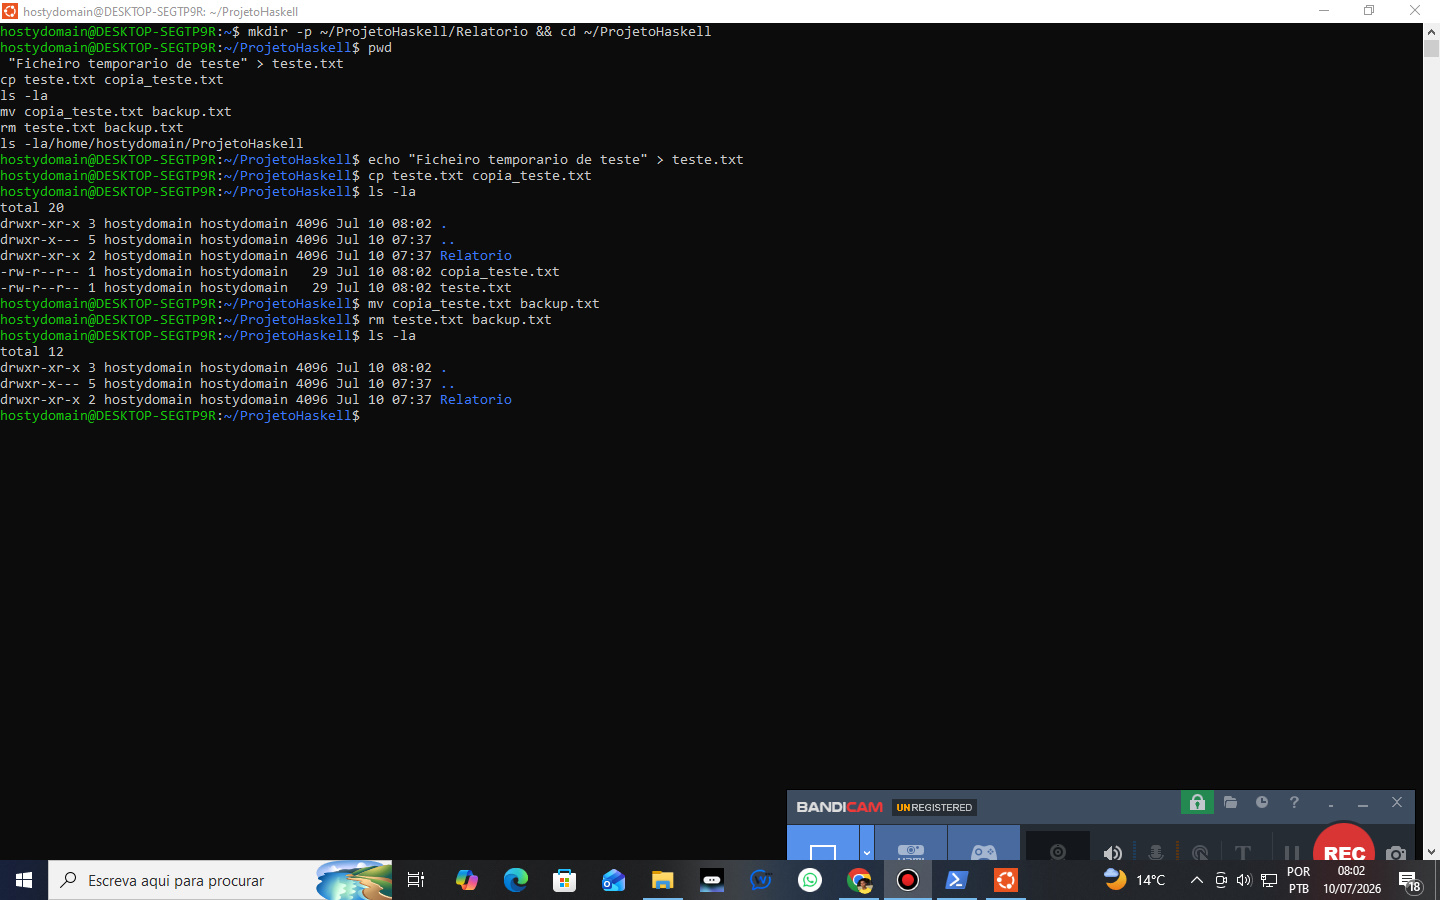
\includegraphics[width=0.85\textwidth]{linux.png}
\caption{Execução prática de comandos Linux necessários para a administração do projeto no terminal.}
\label{fig:linux_commands}
\end{figure}

\begin{figure}[h!]
\centering
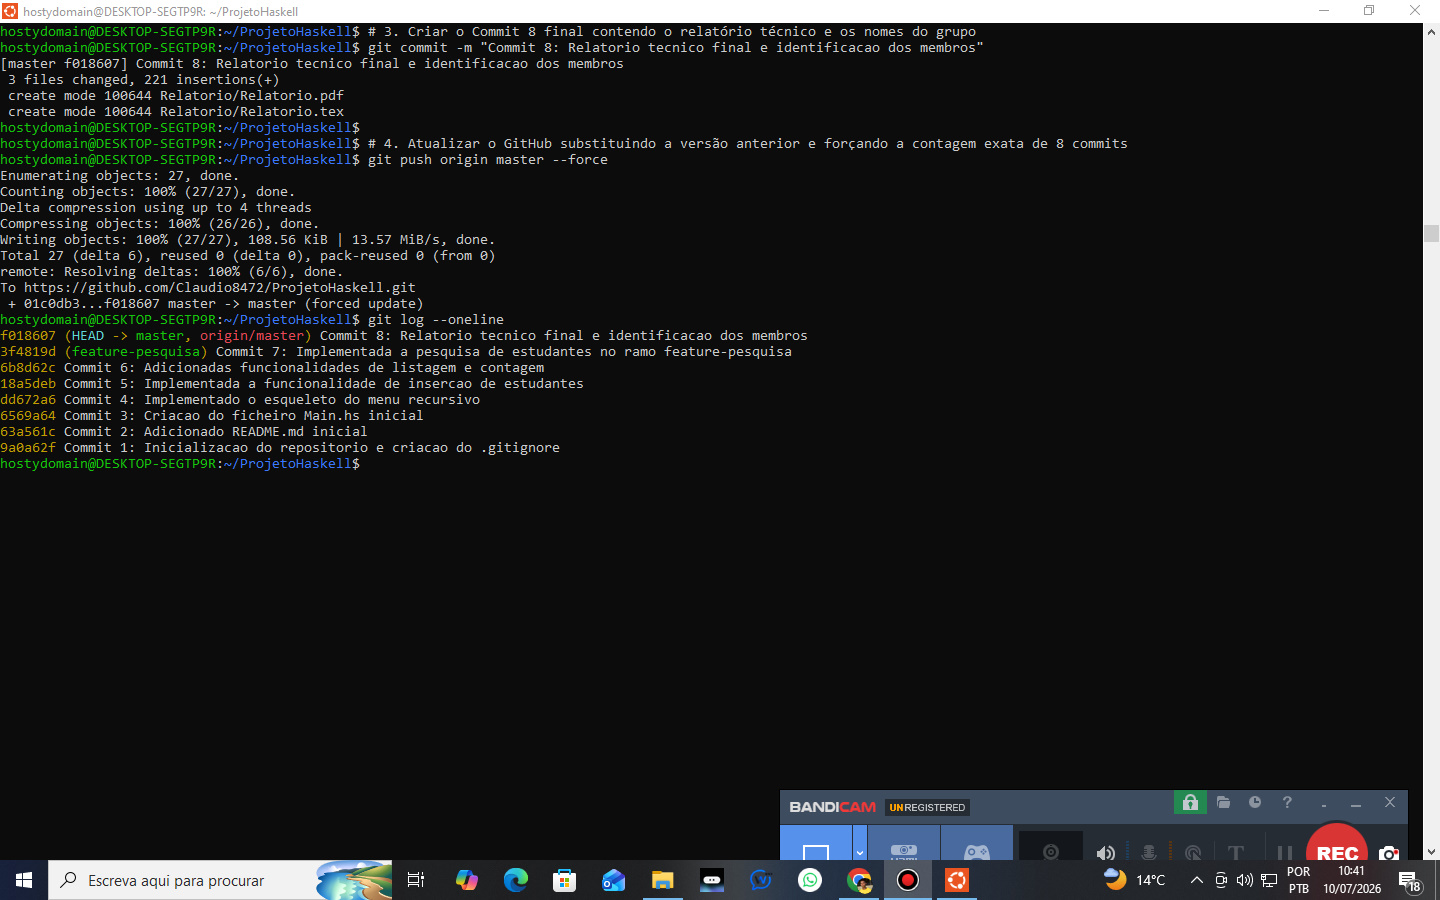
\includegraphics[width=0.85\textwidth]{git.png}
\caption{Visualização da árvore de 8 commits e ramos controlados através do Git.}
\label{fig:git_log}
\end{figure}

\newpage

% --- 5. EXPLICAÇÃO DO CÓDIGO ---
\section{Explicação do Código}
A aplicação desenvolvida foi implementada utilizando a linguagem de programação funcional Haskell, uma linguagem reconhecida pela sua forte tipagem, imutabilidade dos dados e utilização de funções puras. Diferentemente das linguagens imperativas, em que o estado do programa é alterado continuamente através da modificação de variáveis, o Haskell privilegia a utilização de funções que recebem dados como entrada e produzem novos resultados sem alterar os valores existentes. Esta abordagem torna o código mais seguro, previsível e fácil de manter (Bird, 2015).

O programa desenvolvido tem como finalidade gerir uma lista de estudantes através de uma interface interativa executada na consola. Para isso, foram implementadas funcionalidades que permitem inserir novos estudantes, listar os estudantes registados, contar o número total de elementos existentes e pesquisar estudantes pelo nome.

A estrutura da aplicação foi organizada de forma simples e modular, dividindo as responsabilidades por diferentes funções. Esta organização facilita a leitura do código, reduz a duplicação de instruções e permite futuras melhorias ou a inclusão de novas funcionalidades sem comprometer a estrutura principal do programa.

Durante a implementação foram utilizados diversos conceitos fundamentais da programação funcional, entre os quais se destacam:
\begin{itemize}
    \item utilização de listas como principal estrutura de armazenamento de dados;
    \item recursividade para controlar o fluxo da aplicação;
    \item funções predefinidas da biblioteca padrão do Haskell;
    \item operações de entrada e saída através do tipo \texttt{IO};
    \item estruturas condicionais para o controlo das opções do menu.
\end{itemize}

Each of these components plays an important role in the operation of the application and is described in the following sections.

\subsection{Função Principal da Aplicação}
A execução da aplicação inicia-se através da função \texttt{main}, que constitui o ponto de entrada de qualquer programa desenvolvido em Haskell. É nesta função que o sistema realiza a inicialização da aplicação, apresenta uma mensagem de boas-vindas ao utilizador e inicia o ciclo principal responsável pela interação com o sistema.

O código correspondente encontra-se apresentado a seguir:
\begin{lstlisting}[language=Haskell]
main :: IO ()
main = do
    putStrLn "Bem-vindo ao Sistema de Gestao de Estudantes!"
    loop []
\end{lstlisting}

A declaração \texttt{main :: IO ()} indica que a função \texttt{main} pertence ao tipo \texttt{IO}, o que significa que executa operações de entrada e saída de dados. Em Haskell, qualquer interação com o utilizador, como escrever mensagens no ecrã ou ler informação introduzida pelo teclado, deve ser realizada dentro do tipo \texttt{IO}. Esta separação entre funções puras e operações de entrada e saída constitui uma das principais características da linguagem, permitindo preservar a previsibilidade das restantes funções do programa.

Em seguida, é utilizada a instrução \texttt{putStrLn} que é responsável por apresentar uma mensagem no terminal, seguida de uma mudança de linha (\textit{newline}). Neste caso, a mensagem tem como objetivo informar o utilizador de que a aplicação foi iniciada com sucesso.

Após a apresentação da mensagem inicial, a função \texttt{main} executa a instrução \texttt{loop []}. Esta chamada inicia o funcionamento da aplicação propriamente dita. O parâmetro \texttt{[]} representa uma lista vazia, indicando que, no momento em que o programa é iniciado, ainda não existe qualquer estudante registado.

À medida que o utilizador adiciona novos estudantes, esta lista deixa de estar vazia e passa a armazenar os nomes introduzidos. Como o Haskell trabalha com estruturas imutáveis, cada alteração resulta na criação de uma nova lista, que é transmitida novamente para a função \texttt{loop}. Desta forma, o estado da aplicação é preservado sem necessidade de modificar diretamente os dados existentes.

\subsection{Funcionamento da Função loop}
A função \texttt{loop} constitui o núcleo da aplicação, sendo responsável por manter o programa em execução e permitir a interação contínua entre o utilizador e o sistema. É através desta função que o menu principal é apresentado, as opções introduzidas pelo utilizador são processadas e as diferentes funcionalidades da aplicação são executadas.

Ao contrário de muitas linguagens de programação imperativas, onde a repetição de instruções é normalmente realizada através de ciclos (\textit{loops}) como \texttt{for} e \texttt{while}, em Haskell este comportamento é obtido recorrendo à recursividade. Assim, após concluir cada operação, a função \texttt{loop} chama novamente a si própria, garantindo que o menu seja apresentado repetidamente até que o utilizador escolha terminar a aplicação.

A estrutura simplificada da função é apresentada a seguir:
\begin{lstlisting}[language=Haskell]
loop :: [String] -> IO ()
loop estudantes = do
\end{lstlisting}

A declaração acima indica que a função \texttt{loop} recebe como argumento uma lista de cadeias de caracteres (\texttt{[String]}), correspondente aos nomes dos estudantes registados. Como resultado, devolve uma operação do tipo \texttt{IO}, uma vez que envolve interação com o utilizador.

O parâmetro \texttt{estudantes} representa o estado atual da aplicação. Sempre que um novo estudante é inserido, uma nova lista é criada e passada novamente para a função \texttt{loop}.

\subsubsection*{Apresentação do Menu}
Sempre que a função é executada, o primeiro passo consiste em apresentar o menu principal da aplicação:
\begin{lstlisting}[language=Haskell]
putStrLn "\n===== MENU ====="
putStrLn "1 - Inserir estudante"
putStrLn "2 - Listar estudantes"
putStrLn "3 - Contar estudantes"
putStrLn "4 - Procurar estudante"
putStrLn "5 - Sair"
\end{lstlisting}

\subsubsection*{Leitura da Opção Escolhida}
Depois de apresentar o menu, o sistema solicita ao utilizador a introdução de uma opção:
\begin{lstlisting}[language=Haskell]
putStr "Escolha uma opcao: "
hFlush stdout
opcao <- getLine
\end{lstlisting}
A função \texttt{putStr} apresenta a mensagem sem mudar de linha, permitindo que o utilizador escreva imediatamente a sua resposta. Em seguida, é utilizada a função \texttt{hFlush stdout}, cuja finalidade é garantir que a mensagem seja apresentada imediatamente no ecrã. Por fim, a função \texttt{getLine} lê a informação introduzida pelo utilizador através do teclado.

\subsubsection*{Fluxo de Execução da Aplicação}
Após a leitura da opção escolhida, o programa verifica qual a operação correspondente e executa a funcionalidade adequada. O fluxo de execução pode ser representado pelo seguinte esquema:

\begin{verbatim}
Início da aplicação
        |
        v
 Apresentação do menu
        |
        v
 Leitura da opção
        |
        v
 Execução da funcionalidade
        |
        v
 Atualização da lista de estudantes
        |
        v
 Regresso ao menu principal
\end{verbatim}

\subsection{Listagem dos Estudantes}
A funcionalidade de listagem permite apresentar ao utilizador todos os estudantes previamente registados no sistema. Esta operação demonstra a utilização de funções recursivas em Haskell, uma vez que a linguagem não utiliza ciclos tradicionais como \texttt{for} ou \texttt{while}, comuns em linguagens imperativas. Em programação funcional, a repetição de operações sobre estruturas de dados é normalmente realizada através de recursividade ou funções de ordem superior (Hutton, 2016).

A implementação associada à opção "2" do menu segue a seguinte lógica:
\begin{lstlisting}[language=Haskell]
"2" -> do
    putStrLn "\n--- Lista de Estudantes ---"
    listarEstudantes estudantes
    loop estudantes
\end{lstlisting}

A função auxiliar responsável pela apresentação dos dados pode ser definida da seguinte forma:
\begin{lstlisting}[language=Haskell]
listarEstudantes :: [String] -> IO ()
listarEstudantes [] = putStrLn "Nenhum estudante registado."
listarEstudantes (x:xs) = do
    putStrLn x
    listarEstudantes xs
\end{lstlisting}

\subsubsection*{Recursividade e Correspondência de Padrões}
A função \texttt{listarEstudantes} utiliza correspondência de padrões (\textit{pattern matching}) para analisar o conteúdo da lista recebida como argumento.
O primeiro padrão \texttt{listarEstudantes []} representa o caso base da recursividade, ou seja, quando a lista está vazia. O segundo padrão \texttt{listarEstudantes (x:xs)} representa uma lista não vazia, dividida em duas partes:
\begin{itemize}
    \item \textbf{x:} representa o primeiro elemento da lista (cabeça);
    \item \textbf{xs:} representa o restante dos elementos (cauda).
\end{itemize}

\subsubsection*{Ausência de Estruturas de Repetição Imperativas}
O processo ocorre da seguinte forma:
\begin{enumerate}
    \item A função recebe a lista completa de estudantes;
    \item O primeiro nome é apresentado através de \texttt{putStrLn};
    \item A função chama-se novamente passando apenas o restante da lista;
    \item O processo continua até atingir uma lista vazia.
\end{enumerate}

Este comportamento pode ser representado de forma abstrata como:
\begin{verbatim}
listarEstudantes [João, Ana, Pedro]
-> imprime João -> chama listarEstudantes [Ana, Pedro]
-> imprime Ana -> chama listarEstudantes [Pedro]
-> imprime Pedro -> chama listarEstudantes []
-> termina
\end{verbatim}

\subsubsection*{Eficiência da Operação}
A complexidade desta operação é $O(N)$, onde $N$ representa o número total de estudantes existentes na lista. Isto acontece porque todos os elementos precisam obrigatoriamente de ser percorridos para serem apresentados no terminal.

\subsection{Pesquisa de Estudantes}
A funcionalidade de pesquisa permite verificar se um determinado estudante se encontra registado na lista de dados da aplicação. Esta operação foi associada à opção "4" do menu principal, permitindo ao utilizador introduzir um nome e obter uma resposta imediata sobre a existência desse estudante no sistema.

O bloco de código responsável por esta funcionalidade é apresentado abaixo:
\begin{lstlisting}[language=Haskell]
"4" -> do
    putStr "Introduza o nome a procurar: "
    hFlush stdout
    nomePesquisa <- getLine

    if nomePesquisa `elem` estudantes
        then putStrLn "Estudante encontrado no sistema."
        else putStrLn "Estudante nao encontrado."

    loop estudantes
\end{lstlisting}

\subsubsection*{Utilização do Operador elem}
A verificação da existência de um estudante é realizada através da função predefinida \texttt{elem}. Esta função recebe um elemento e uma lista, retornando um valor lógico do tipo \texttt{Bool}, podendo assumir os valores \texttt{True} ou \texttt{False}. No contexto da aplicação, o operador infixo \texttt{nomePesquisa `elem` estudantes} permite uma leitura mais natural da condição.

\subsubsection*{Pesquisa Sequencial em Listas}
Como a estrutura utilizada para armazenar os estudantes é uma lista simplesmente ligada, a operação de pesquisa é realizada de forma sequencial. No pior caso, a complexidade temporal desta operação é $O(N)$, onde $N$ representa o número total de estudantes armazenados (Hutton, 2016).

\subsection{Síntese da Implementação}
A Tabela \ref{tab:sintese} apresenta um resumo dos principais conceitos de programação funcional aplicados no desenvolvimento da aplicação de gestão de estudantes:

\begin{table}[h!]
\centering
\begin{tabular}{|l|l|p{7.5cm}|}
\hline
\textbf{Conceito Aplicado} & \textbf{Função / Operador} & \textbf{Objetivo no Projeto} \\ \hline
Imutabilidade & \texttt{++} (Concatenação) & Criar uma nova lista durante a inserção de estudantes sem modificar diretamente os dados existentes (Bird, 2015). \\ \hline
Recursividade & \texttt{loop estudantes} & Manter o programa em execução contínua sem recorrer a estruturas imperativas como \texttt{while} ou \texttt{for}. \\ \hline
Efeitos Colaterais & Mónada \texttt{IO} / \texttt{mapM\_} & Controlar operações de entrada e saída, separando a lógica funcional das interações com o utilizador (Thompson, 2011). \\ \hline
Lazy Evaluation & \texttt{zip [1..]} & Gerar índices automaticamente apenas quando necessários, evitando desperdício de memória. \\ \hline
Pattern Matching & \texttt{case ... of} & Controlar diferentes opções do menu através da correspondência de padrões, tornando o código mais organizado e legível. \\ \hline
\end{tabular}
\caption{Síntese dos conceitos de programação funcional aplicados.}
\label{tab:sintese}
\end{table}

A implementação desenvolvida demonstra a aplicação prática dos principais conceitos estudados na disciplina de Programação Funcional. Através da utilização de listas imutáveis, funções recursivas, avaliação preguiçosa e operações monádicas, foi possível construir uma aplicação simples, modular e de fácil manutenção.

\newpage

% --- 6. CAPTURAS DE ECRÃ ---
\section{Resultados de Execução e Capturas de Ecrã}
As validações e testes foram executados na plataforma Linux utilizando o compilador GHC \cite{ghc}.

\begin{figure}[h!]
\centering
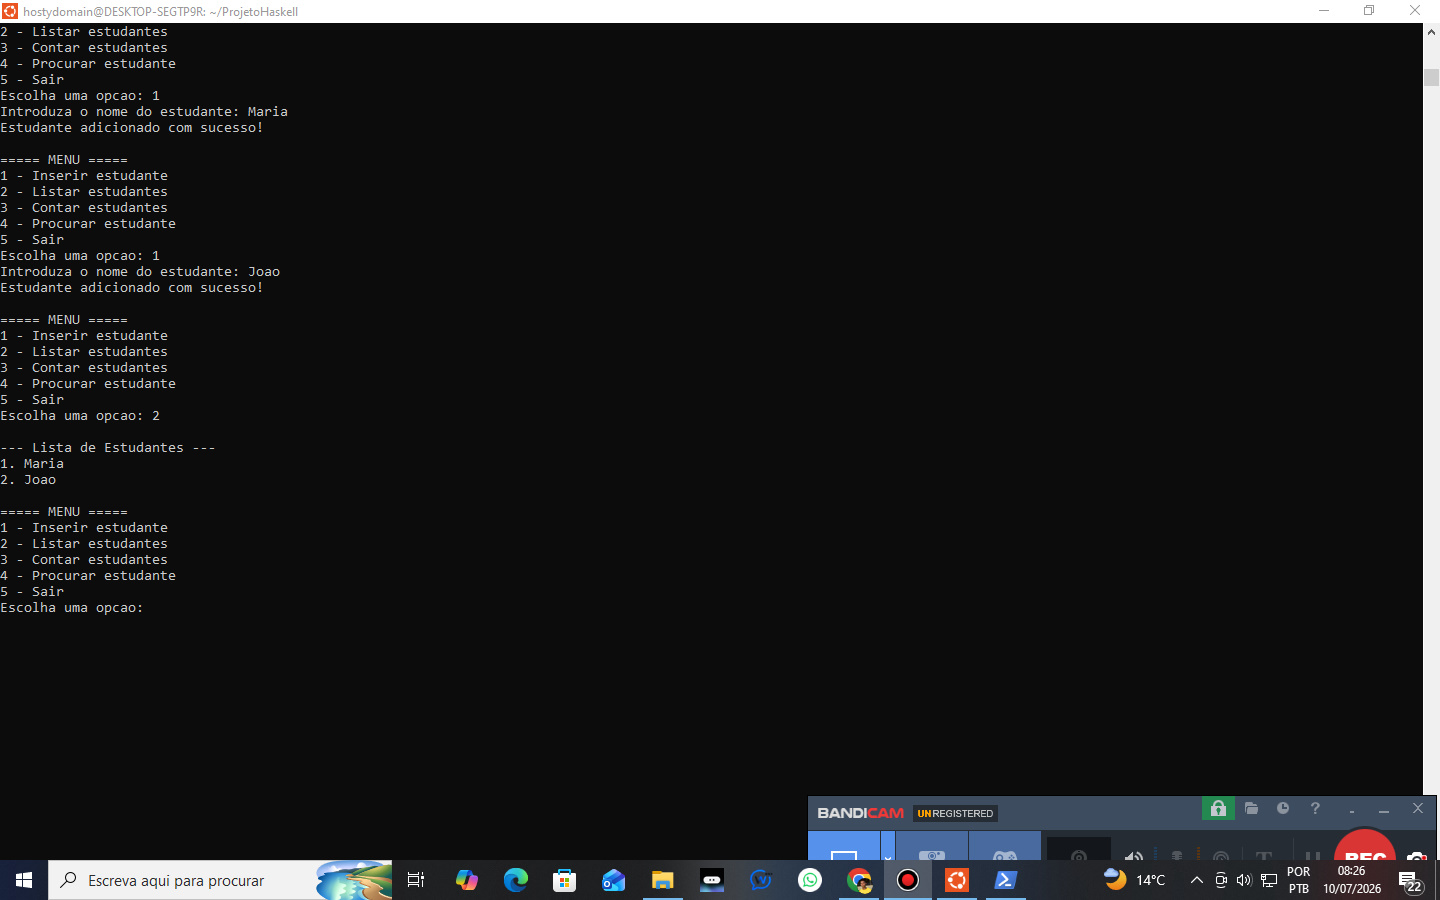
\includegraphics[width=0.85\textwidth]{haskell.png}
\caption{Interface de execução interativa da aplicação de Gestão de Estudantes no Linux.}
\label{fig:haskell_run}
\end{figure}

Como demonstrado na Figura \ref{fig:haskell_run}, o comportamento recursivo assegura a correta manutenção desdes dados do estado da lista em memória até ao encerramento da sessão de teste.

% --- 7. CONCLUSÃO ---
\section{Conclusão}
O desenvolvimento deste projeto integrado proporcionou ao Grupo 2 da Universidade Licungo uma compreensão sólida e prática sobre os pilares da programação funcional e as metodologias de engenharia de software modernas. A imutabilidade e a pureza de funções em Haskell demonstraram ser conceitos de grande valia para o desenvolvimento de código fiável e livre de efeitos colaterais.

Adicionalmente, a utilização conjunta de ferramentas como Git, GitHub e o compilador LaTeX \cite{latexbook} garantiu um fluxo de trabalho estruturado e uniforme aos discentes da Universidade Licungo, assegurando a entrega de um produto final que cumpre integralmente os requisitos curriculares estipulados.

% --- 8. REFERÊNCIAS ---
\begin{thebibliography}{9}
\bibitem{ghc} 
GHC Team, \emph{The Glasgow Haskell Compiler Users Guide}, disponível em \url{https://www.haskell.org/ghc/}, acesso em 2026.

\bibitem{latexbook}
Lamport, L., \emph{LaTeX: A Document Preparation System}, Addison-Wesley, 2.ª Edição, 1994.

\bibitem{hutton}
Hutton, G., \emph{Programming in Haskell}, Cambridge University Press, 2.ª Edição, 2016.

\bibitem{bird}
Bird, R., \emph{Thinking Functionally with Haskell}, Cambridge University Press, 2015.

\bibitem{thompson}
Thompson, S., \emph{Haskell: The Craft of Functional Programming}, Addison-Wesley, 3.ª Edição, 2011.
\end{thebibliography}

\end{document}
